%==========================================================================
%  TRES0312 Fysikk — Foiler-mal
%
%  MØrk/lys modus: kommenter ut én av de to linjene nedenfor.
%==========================================================================
\newif\ifdarkmode
\darkmodetrue      % ← mørk modus
%\darkmodefalse   % ← lys modus  (fjern % foran og legg % foran linjen over)

\documentclass[aspectratio=169, 12pt]{beamer}

\usepackage{amd-beamer}
\usetikzlibrary{overlay-beamer-styles}   % for "visible on=<->" i enkelte tikz-figurer
\usetikzlibrary{calc}   % for tikz-overlayet på Håland-figuren (forside)

%--------------------------------------------------------------------------
%  Farger hentet fra kompendiets amd.sty (ikke definert i amd-beamer.sty),
%  brukt av tikz-overlayet på straffespark-figuren (forsiden).
%--------------------------------------------------------------------------
\definecolor{mycolor}{RGB}{38,168,148}
\definecolor{exmscol}{HTML}{e04b52}

%--------------------------------------------------------------------------
%  \imgpt{navn}{xfrac}{yfrac} -- definert HER (utenfor enhver frame), siden
%  beamer fanger opp hele frame-innholdet for overlay-avspilling; en
%  \newcommand med #1/#2/#3 inne i en frame gir "Illegal parameter number".
%--------------------------------------------------------------------------
\newcommand{\imgpt}[3]{%
    \coordinate (#1tmpx) at ($(img.south west)!#2!(img.south east)$);%
    \coordinate (#1tmpy) at ($(img.south west)!#3!(img.north west)$);%
    \coordinate (#1) at (#1tmpx |- #1tmpy);%
}

%--------------------------------------------------------------------------
%  DOKUMENTINFO
%--------------------------------------------------------------------------
\title{Kinematikk}
\subtitle{TRES0312 --- Prosjektilbevegelse}
\author{Ben David Normann}
\date{\today}

%--------------------------------------------------------------------------
%  SEKSJONSKONTEKST
%  \setcounter{section}{N} setter gjeldende seksjonsnummer til N, slik at
%  \defn, \exm og \oppgave får samme nummerering som i kompendiet.
%  Tellerne nullstilles automatisk ved hvert \setcounter{section}{...}.
%--------------------------------------------------------------------------
\setcounter{section}{3}   % Kapittel 3: "Kinematikk"

\begin{document}

%--------------------------------------------------------------------------
%  SLIDE 1 — TITTELSIDE
%--------------------------------------------------------------------------
\begin{frame}[plain]
  \titlepage
  \dekkerdelkapoverlay{kapittel 3.4}

  % Håland-figuren (med tikz-overlay fra kompendiets Figur 3.7) som ren
  % illustrasjon nederst på forsiden -- ingen figurtekst.
  \begin{tikzpicture}[remember picture, overlay]
    \node[anchor=north, inner sep=0pt] at ($(current page.north)+(0,-4.1cm)$) {%
      \scalebox{0.65}{%
      \begin{tikzpicture}
      \node[anchor=south west, inner sep=0pt] (img) at (0,0) {%
        \ifdarkmode
          
\includegraphics[width=10cm]{Images/Straffespark_Haaland_transp_mork.png}
        \else
          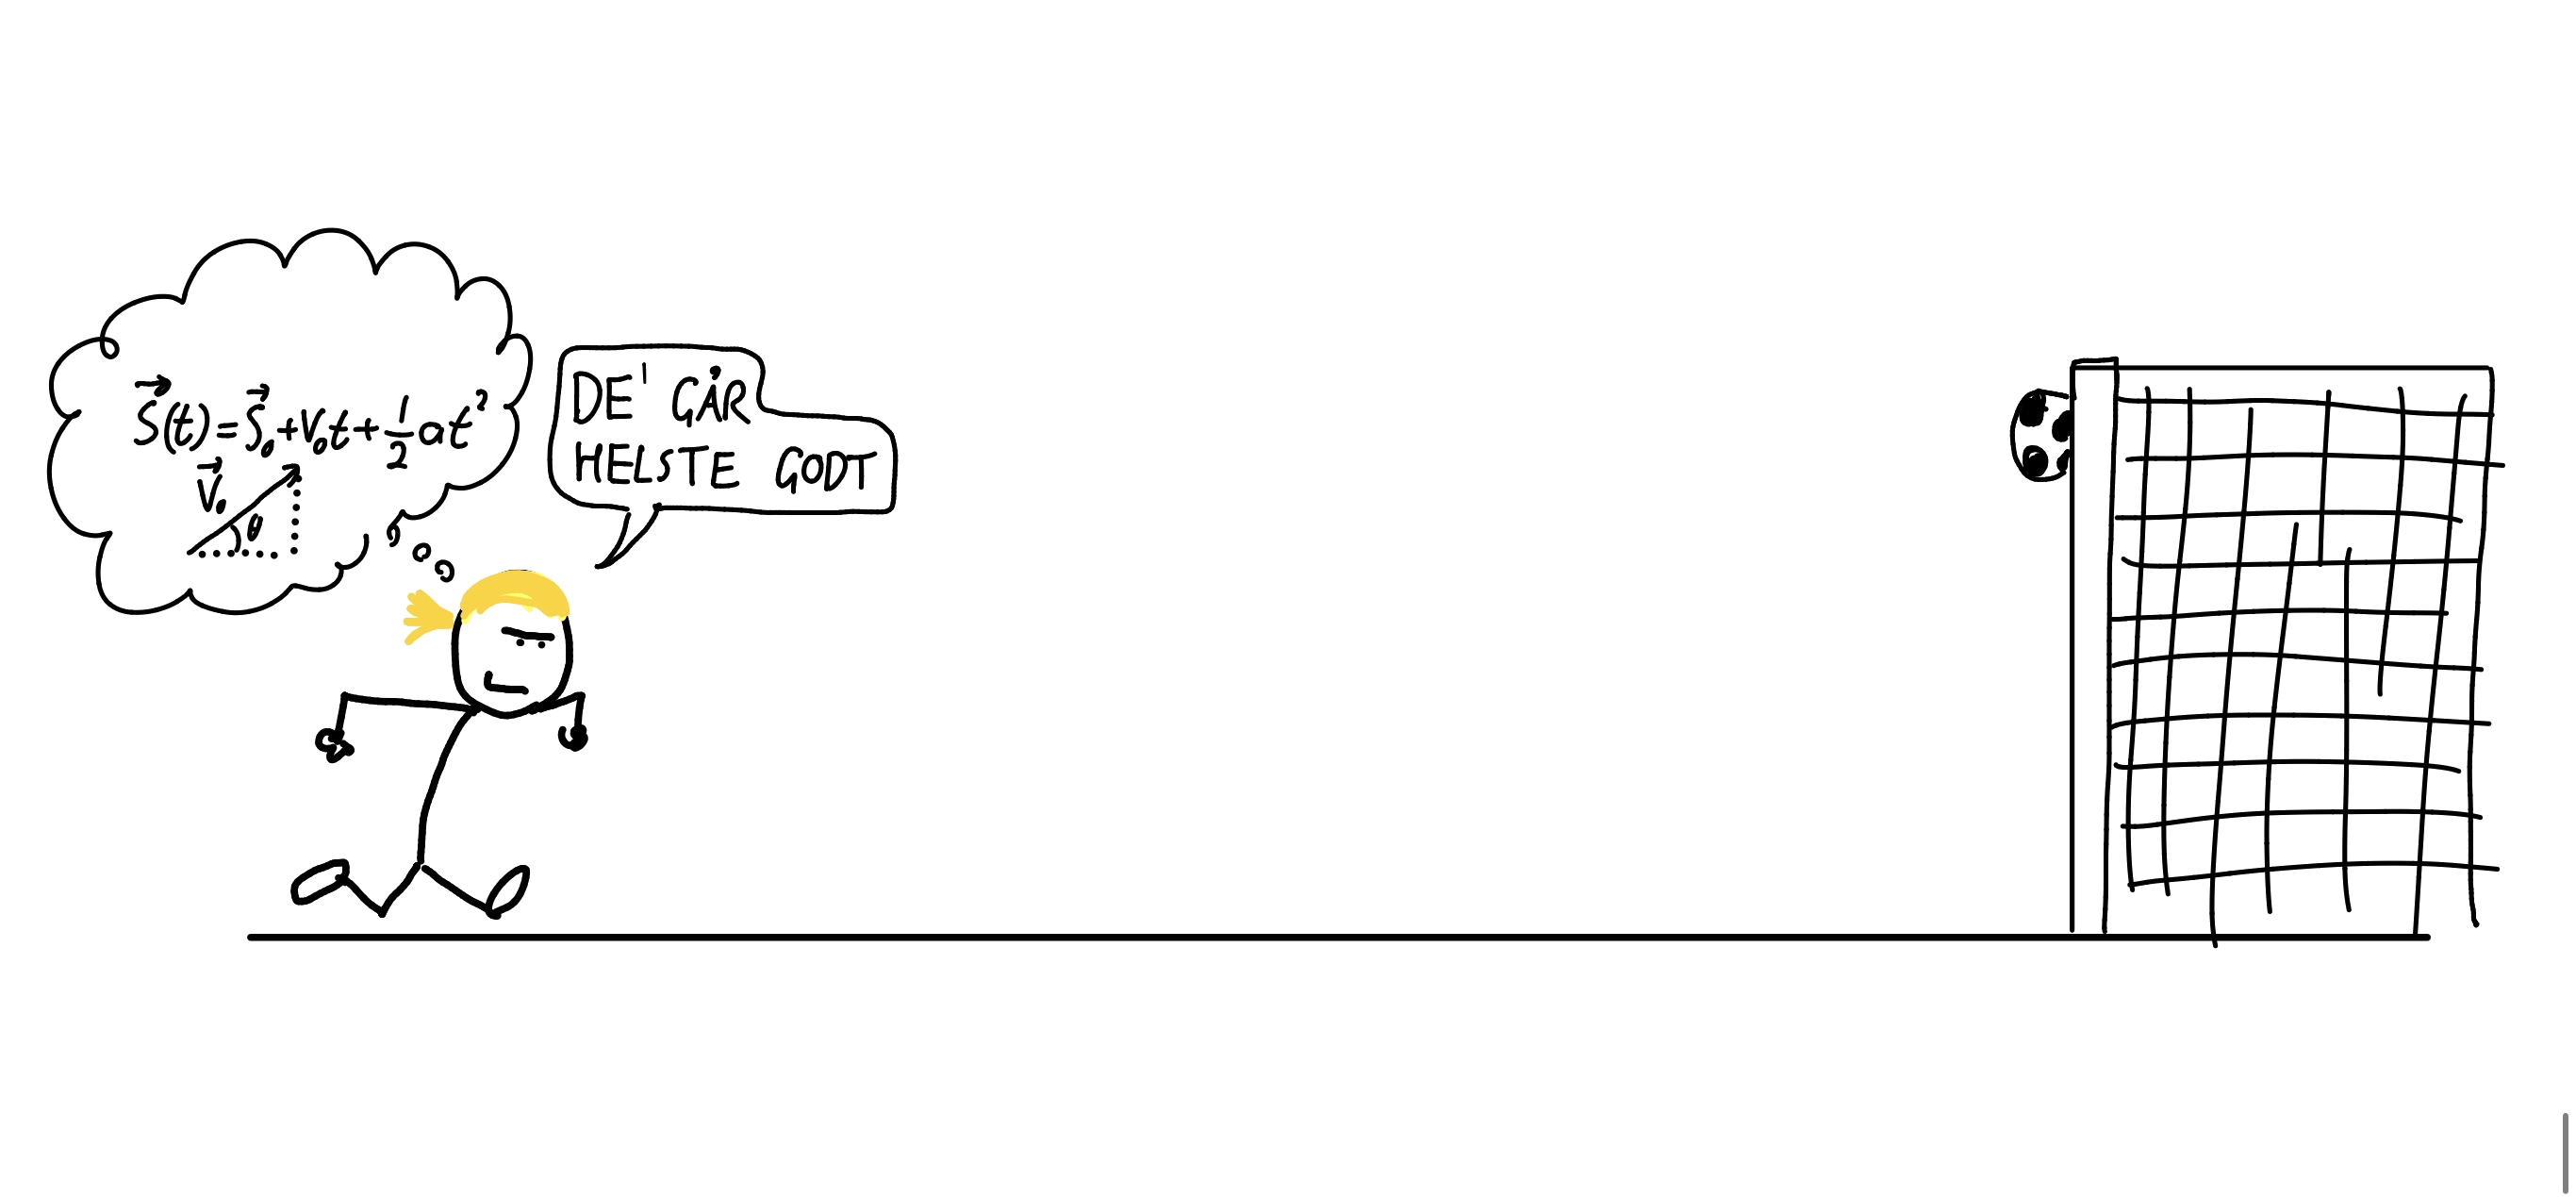
\includegraphics[width=10cm]{Images/Straffespark_Haaland_transp_lys.png}
        \fi
      };
      \imgpt{Foot}{0.213}{0.278}
      \imgpt{Ball}{0.757}{0.653}
      \imgpt{FootGround}{0.213}{0.2175}
      \imgpt{PostGround}{0.798}{0.2175}
      \imgpt{Hleft}{0.213}{0.16}
      \imgpt{Hright}{0.798}{0.16}
      \imgpt{Vbottom}{0.68}{0.2175}
      \imgpt{Vtop}{0.68}{0.653}
      \imgpt{Hlabel}{0.5055}{0.13}
      \imgpt{Vlabel}{0.625}{0.435}
      \imgpt{Traj0}{0.2130}{0.2780}
      \imgpt{Traj1}{0.2493}{0.3408}
      \imgpt{Traj2}{0.2855}{0.3982}
      \imgpt{Traj3}{0.3218}{0.4502}
      \imgpt{Traj4}{0.3581}{0.4968}
      \imgpt{Traj5}{0.3943}{0.5380}
      \imgpt{Traj6}{0.4306}{0.5739}
      \imgpt{Traj7}{0.4669}{0.6043}
      \imgpt{Traj8}{0.5031}{0.6293}
      \imgpt{Traj9}{0.5394}{0.6489}
      \imgpt{Traj10}{0.5757}{0.6630}
      \imgpt{Traj11}{0.6119}{0.6718}
      \imgpt{Traj12}{0.6482}{0.6752}
      \imgpt{Traj13}{0.6845}{0.6732}
      \imgpt{Traj14}{0.7207}{0.6658}
      \draw[dashed, very thick, exmscol]
        (Traj0) -- (Traj1) -- (Traj2) -- (Traj3) -- (Traj4) -- (Traj5) -- (Traj6) -- (Traj7)
        -- (Traj8) -- (Traj9) -- (Traj10) -- (Traj11) -- (Traj12) -- (Traj13) -- (Traj14) -- (Ball);
      \draw[dotted, textcolor!60] (Foot) -- ($(Foot)+(1.6,0)$);
      \draw[->, very thick, exmscol] (Foot) -- ++(40:1.6) node[above right=1pt, exmscol] {\large $\vec{v}_0$};
      \draw[textcolor!70] ($(Foot)+(0.7,0)$) arc (0:40:0.7);
      \node[font=\small, textcolor!70] at ($(Foot)+({0.95*cos(20)},{0.95*sin(20)})$) {$\theta$};
      \draw[<->, thick, mycolor] (Hleft) -- (Hright);
      \draw[dotted, mycolor!50] (FootGround) -- (Hleft);
      \draw[dotted, mycolor!50] (PostGround) -- (Hright);
      \node[below=2pt, mycolor] at (Hlabel) {\large $11\,\text{m}$};
      \draw[<->, thick, mycolor] (Vbottom) -- (Vtop);
      \draw[dotted, mycolor!50] (Vtop) -- (Ball);
      \node[left=2pt, mycolor] at (Vlabel) {\large $2.30\,\text{m}$};
      \end{tikzpicture}%
      }%
    };
  \end{tikzpicture}
\end{frame}

%--------------------------------------------------------------------------
%  SLIDE 2 — Aktivitet fra forrige gang: Fart-strekning-likningen
%  (Slide 9 i F5 — vi rakk den ikke.)
%--------------------------------------------------------------------------
\begin{frame}{Aktivitet}

  \aktivitet{Fart-strekning-likningen}{%
  En bil øker farten fra $v_0 = 5\,\mathrm{m/s}$ til $v = 25\,\mathrm{m/s}$ i løpet av $t = 4\,\mathrm{s}$.
  Bestem strekningen $s$ bilen har tilbakelagt.
  }

\end{frame}

%--------------------------------------------------------------------------
%  SLIDE 3 — Aktivitet fra forrige gang: Fritt fall
%  (Slide 8 i F5 — vi rakk den ikke.)
%--------------------------------------------------------------------------
\begin{frame}{Aktivitet}

  \aktivitet{Fritt fall}{%
  \begin{enumerate}[a)]
      \item En sten kastes rett oppover, og faller rett ned igjen. Hva er akselerasjonen til steinen (i) på vei opp, (ii) på toppen og (iii) på vei ned? Tegn figur og forklar kort med ord.
    \item Tegn (kvalitativt) grafene $a(t)$, $v(t)$ og $s(t)$ for bevegelsen i a)ii) (steinen som kastes rett oppover).
  \end{enumerate}
  }

\end{frame}

%--------------------------------------------------------------------------
%  SLIDE 4 — Repetisjon: a = konst., og dekomponering i x- og y-retning
%--------------------------------------------------------------------------
\begin{frame}{}

  \begin{columns}[T]
    %--- Venstre: de fire likningene (samlet, som i F5 slide 5) ---
    \begin{column}{0.30\textwidth}
      \centering
      {\Large $\vec{a} = \text{konst.}$}\\[10pt]
      \footnotesize
      $\displaystyle
      \left\{\begin{array}{l}
        \vec{v} = \vec{v}_0 + \vec{a}\,t \\[10pt]
        \vec{s} = \vec{s}_0 + \vec{v}_0\,t + \tfrac{1}{2}\vec{a}\,t^2 \\[10pt]
        |\vec{v}|^2 = |\vec{v}_0|^2 + 2\,\vec{a}\cdot(\vec{s}-\vec{s}_0) \\[10pt]
        \vec{s}-\vec{s}_0 = \dfrac{\vec{v}_0+\vec{v}}{2}\,t
      \end{array}\right.$
    \end{column}
    \pause
    %--- Skillelinje 1 ---
    \begin{column}{0.02\textwidth}
      \centering
      \ifdarkmode\color{white!25!gray}\else\color{black!20}\fi
      \rule{0.4pt}{4.3cm}
    \end{column}
    %--- Midten: dekomponering i x-retning ---
    \begin{column}{0.32\textwidth}
      \centering
      {\large\bfseries $x$-retning}\\[10pt]
      \footnotesize
      $\displaystyle
      \left\{\begin{array}{l}
        v_x = v_{0x} + a_x\,t \\[14pt]
        s_x = s_{0x} + v_{0x}\,t + \tfrac{1}{2}a_x\,t^2
      \end{array}\right.$
    \end{column}
    \pause
    %--- Skillelinje 2 ---
    \begin{column}{0.02\textwidth}
      \centering
      \ifdarkmode\color{white!25!gray}\else\color{black!20}\fi
      \rule{0.4pt}{4.3cm}
    \end{column}
    %--- Høyre: dekomponering i y-retning ---
    \begin{column}{0.32\textwidth}
      \centering
      {\large\bfseries $y$-retning}\\[10pt]
      \footnotesize
      $\displaystyle
      \left\{\begin{array}{l}
        v_y = v_{0y} + a_y\,t \\[14pt]
        s_y = s_{0y} + v_{0y}\,t + \tfrac{1}{2}a_y\,t^2
      \end{array}\right.$
    \end{column}
  \end{columns}

\end{frame}

%--------------------------------------------------------------------------
%  SLIDE 5 — Aktivitet: Kanon (prosjektilbevegelse)
%--------------------------------------------------------------------------
\begin{frame}{Aktivitet}

  \begin{columns}[T]
    \begin{column}{0.40\textwidth}
      \aktivitet{Kanonen}{%
      En kanon skyter en kule fra en høyde $y_0 = 0.25\,\mathrm{m}$ over bakken, med en vinkel på $60^\circ$ i forhold til horisontalen. Utgangsfarten til kula er $v_0 = 4.84\,\mathrm{m/s}$.
      \begin{enumerate}[a)]
        \item Finn startfarten dekomponert i $x$- og $y$-retning.
        \item Bestem hvor lang tid kula er i lufta før den lander.
        \item Bestem hvor langt bort kula lander (horisontal avstand).
      \end{enumerate}
      }
    \end{column}
    \begin{column}{0.56\textwidth}
      \centering
      \ifdarkmode
        
\includegraphics[width=\linewidth]{Images/Prosjektilbevegelse_skisse_mork.png}
      \else
        
\includegraphics[width=\linewidth]{Images/Prosjektilbevegelse_skisse_lys.png}
      \fi
      \vspace{4pt}
      {\tiny Python: \texttt{TRES0312 Python/Kap3\_Kinematikk/K3\_prosjektilbevegelse\_kanon.ipynb}}
    \end{column}
  \end{columns}

\end{frame}

%--------------------------------------------------------------------------
%  SLIDE 6 — Neste gang
%--------------------------------------------------------------------------
\begin{frame}
\begin{center}
  \Huge{Neste gang: Plenumsregning}
  \begin{itemize}
    \item Vi går sammen gjennom flere oppgaver i kinematikk
    \item Både 1D-bevegelse og 2D-bevegelse (prosjektilbevegelse)
  \end{itemize}
\end{center}
\end{frame}

\end{document}
